\documentclass{llncs}
\usepackage[utf8]{inputenc}
\usepackage{graphicx}
\usepackage{amsmath}
\usepackage{verbatim}
\usepackage[T2A]{fontenc}
\title{Feature Engineering and Gradient Boosting in the Discovery Challenge}
\author{Andrey Zimovnov \and Evgeny Sokolov}
\institute{Yandex Data Factory}

\begin{document}
	
	\maketitle
	
	\section{Introduction}
	
	Customers generate large amounts of unstructured data every day. Such data can bring a great value to a business, but extracting this value is a complex data mining problem. A typical example is a bank, where customers create transactional data on payments, visits, etc. These data can be used for scoring, fraud detection, recommender systems and lots of other tasks, but classical machine learning algorithms cannot incorporate transactional features directly~— they should be transformed into numerical or categorical features first.
	
	The ECML/PKDD 2016 Discovery Challenge is organized around two typical examples of such problems. We are given a two year trace of card payment events with geo location information and have two goals:
	\begin{enumerate}
		\item Predict 5 bank branches that the user visits most often.
		\item Predict whether the user will apply for a credit card during a certain period.
	\end{enumerate}
	
	Our solution consists of several steps. Firstly, we analyze the quality metrics and reduce both problems to a series of binary classification tasks. Secondly, we propose a number of features based on transactional data provided. Thirdly, we select the best model for each problem.
	
	\section{Data Description}
	
	The challenge consists of two supervised learning tasks. For both, we are given information on a set of users from 2014 for training with the actual target labels. Evaluation is done on another, completely different set of users. For these, we are given information for the first half of 2015. In both tasks we are asked to predict user behavior for the second half of 2015 for each test user \cite{competition_page}.
	
	\subsection{User Info Data}
	
	\begin{enumerate}
		\item \verb|USER_ID| -- Unique user ID.
		\item \verb|AGE_CAT| -- Age category (a = $\le$35, b = 36--65, c = >65).
		\item \verb|LOC_CAT| -- Location category of the user (a = capital, b = city, c = village).
		\item \verb|INC_CAT| -- Income category (a = low, b = medium, c = high, d = no income).
		\item \verb|GEN| -- Gender (1 = male, 0 = female).
		\item \verb|LOC_GEO_X| -- Geo info of user address is rounded to 100m.
		\item \verb|LOC_GEO_Y| -- Geo info of user address is rounded to 100m.
		\item \verb|TARGET_TASK_2| -- The date when the user applied for credit card. Only given for training users.
		\item \verb|C201*| -- Binary columns for each month. If True, the user has at least one credit card.
		\item \verb|W201*| -- Binary columns for each month. If True, the user is categorized as "wealthy" in the system of the bank.
	\end{enumerate}
		
	\begin{figure}[h]
		\centering
		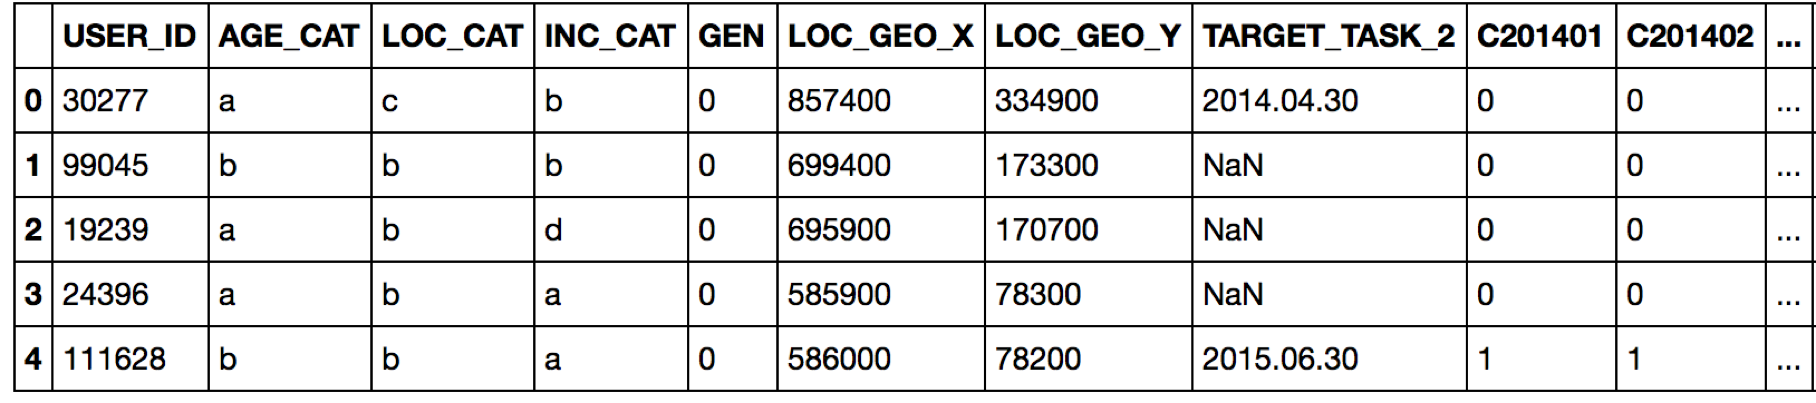
\includegraphics[width=\textwidth]{user_data}
		\caption{Sample of user info data.}
		\label{user_data}
	\end{figure}
	
	\subsection{Transaction Data}
	
	\begin{enumerate}
		\item \verb|USER_ID| -- Unique user ID.
		\item \verb|POI_ID| -- Unique shop ID.
		\item \verb|CHANNEL| -- Type of activity (p = pos, n = webshop, b = branch).
		\item \verb|DATE| -- Date of activity.
		\item \verb|TIME_CAT| -- Time (rounded to a = 05--11h, b = 12--18h, c = 19--04h).
		\item \verb|LOC_CAT| -- Event location category (a = capital, b = city, c = village).
		\item \verb|MC_CAT| -- Anonymized market category groups (types are indexed from a to j).
		\item \verb|CARD_CAT| -- Credit vs. debit card (c = credit card, d = debit card).
		\item \verb|AMT_CAT| -- Amount of money spent in three categories (a = low, b = medium, c = high).
		\item \verb|GEO_X| -- Geolocation information of the event.
		\item \verb|GEO_Y| -- Geolocation information of the event.
	\end{enumerate}
	
	\begin{figure}[h]
		\centering
		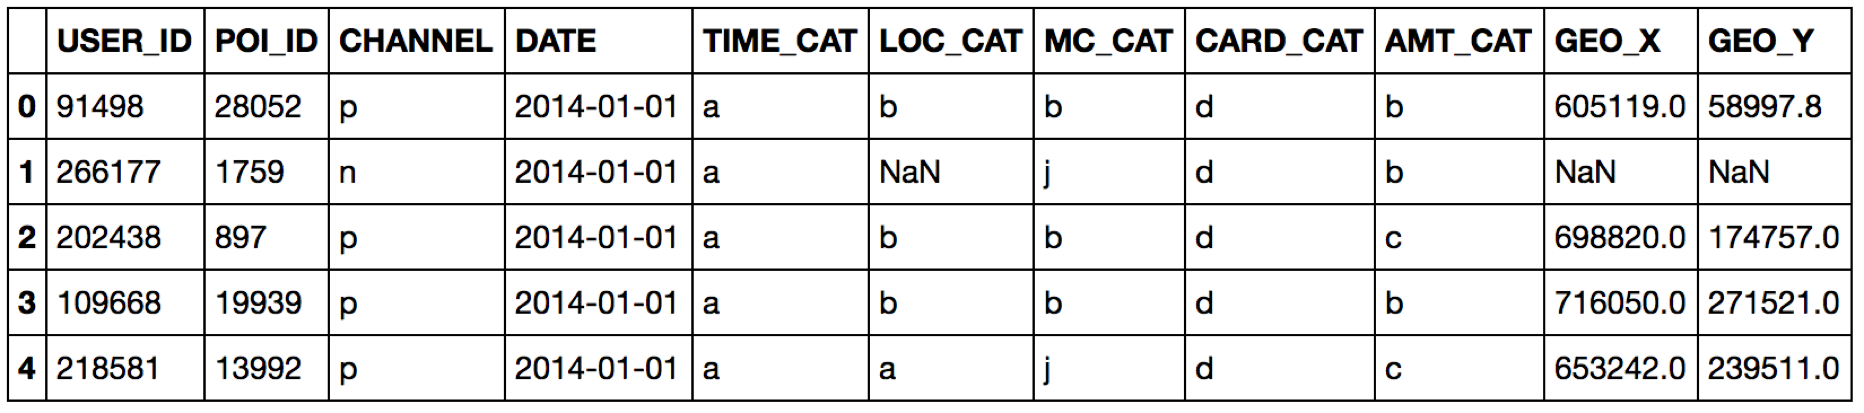
\includegraphics[width=\textwidth]{transaction_data}
		\caption{Sample of transaction data.}
		\label{transaction_data}
	\end{figure}
	
	\section{Task 1: Predict the bank branches visited by the user}
	
	In this task we are asked to predict 5 out of 323 bank branches that the user visits most often. The solution is evaluated by the mean of the average of $cosine@1$ and $cosine@5$ for all users, where $cosine@k$ is defined by
	$$
	cosine@k = \frac{\sum_{i=1}^{k}v(p_i)\hat{v}(p_i)}{\sqrt{\sum_{j} v(j)^2} \sqrt{\sum_{i=1}^{k} \hat{v}(p_i)^2}},
	$$
	where $v(i)$ notes the actual number of visits of the branch $i$, $\hat{v}(j)$ notes the predicted number of visits of the branch $j$, and $p_1, \dots, p_5$ ($\hat{v}(p_1) \ge \ldots \ge \hat{v}(p_5)$) are the indexes of the most visited branches by the user.
	
	\subsection{Engineered Features} \label{features_1_section}
	
	\subsubsection{User Features.}
	
	For each user $u$ we define a feature vector $f_u$, which is a concatenation of the following vectors:
	\begin{enumerate}
		\item Euclidean distances from the user geo location to all of the 323 bank POIs' geo locations.
		\item C201* features for the first 6 months (binary columns for each month, if True, the user has at least one credit card).
		\item W201* features for the first 6 months (binary columns for each month, if True, the user is categorized as "wealthy" in the system of the bank).
		\item Gender, age, income, location categories one-hot encoded vectors.
	\end{enumerate}
	
	\subsubsection{User's Transactions Features.}
	For each user $u$ we also define a feature vector $f_{ut}$ based on user's transactions for the first 6 months.
	
	Each transaction is characterized by time category, location category, merchant category, card category and amount category. For any set of above features we can define a vector of counters \cite{mscounts} for all possible value combinations. For instance, let's take into consideration card category and amount category, which can take $(c, d, \emptyset)$ and $(a, b, c, \emptyset)$ values respectively. For them we define counters for any possible values combination $(c, a)$, $(c, b)$, \dots, $(\emptyset, c)$, $(\emptyset, \emptyset)$. For each combination corresponding counter is incremented with every transaction having such values combination. We'll refer to the resulting vector of counters as $C$(card, amount) for the example above.
	
	Each transaction also has a geo location, we propose to use it to count how many transactions took place next to the nearest bank POI, i.e. we increment bank POI counter each time it is the nearest to a transaction geo location. This way we acquire a vector $L$ of counters of length 323.
	
	The resulting vector $f_{ut}$ is then defined as a concatenation of the following vectors:
	\begin{enumerate}
		\item $C$(time)
		\item $C$(location)
		\item $C$(merchant)
		\item $C$(card)
		\item $C$(amount)
		\item $C$(merchant, amount)
		\item $C$(location, merchant)
		\item $C$(time, location, amount)
		\item $C$(card, amount)
		\item $C$(merchant, card, amount)
		\item $L$
	\end{enumerate}
	
	\subsection{Proposed method}
	
	For each user in the training set we calculate $f_u$ and $f_{ut}$ features and concatenate them to form a row vector $x_u$, this way obtaining a feature matrix $X$. For each user $u$ we define a row vector $y_u$ of length 323 that contains how many times a user visited one of the 323 bank POI's in the second 6 months of training. All the vectors $y_u$ are stacked in the matrix $Y$.
	
	We decided to go with holdout set for evaluation. We took 10\% of users for testing. This scheme correlated with the public leaderboard and gave us an opportunity to make our experiments faster compared to K-fold cross-validation.
	
	Our task was to predict the values in $y_u$ vectors for the test users. For that task we trained 323 binary classifiers on $X$, where each classifier $c_i$, $i=1,\ldots,323$ predicts if the user will visit bank POI with index $i$ or not. For each classifier $c_i$ we took users, who visited bank POI with index $i$ at least once as positive examples, and all the other users as negative examples. Every classifier is gradient boosted decision trees \cite{fgb} implemented in xgboost. We tuned the number of trees using cross-validation on the training set, the optimal value was around $75 \pm 25$, but most of them had 75, so we took 75 trees for each bank POI to avoid overfitting.
	
	At testing time we applied 323 classifiers $c_i$ and obtained probabilities of positive class $p_i$ from each of them. Bank branches were ranked by the predicted probabilities $\hat{y}_u = [p_1, p_2, \ldots, p_{323}]$, and this ranking was used as a final answer. Although the probabilities from different classifiers are not calibrated and it's not really a good thing to compare probabilities from different classifiers, it proved to work better than other approaches that we tried, including pairwise mode in xgboost and multi-class classification of the most visited bank POI.
	
	\section{Task 2: Upselling prediction}
	
	If the client has debit card only, the client may apply for a credit card (upselling).
	Out task is to predict for all users in the test set if she applies for a credit card in the testing period.
	The predictions are evaluated by Area Under Curve (AUC).
	
	\subsection{Engineered Features}
	
	\subsubsection{User Features.}
	
	For each user $u$ we define a feature vector $f_u$, which is a concatenation of the following vectors:
	\begin{enumerate}
		\item Two geo location coordinates of the user.
		\item Euclidean distance from the user to mean geo location (which is roughly the capital of the country).
		\item C201* features for the first 6 months (binary columns for each month, if True, the user has at least one credit card).
		\item W201* features for the first 6 months (binary columns for each month, if True, the user is categorized as "wealthy" in the system of the bank).
		\item Gender, age, income, location categories one-hot encoded vectors.
	\end{enumerate}
	
	\subsubsection{User's Transactions Features.}
	For each user $u$ we also define a feature vector $f_{ut}$ based on user's transactions for the first 6 months.
	
	We use almost the same counter features that were described in section \ref{features_1_section}, for example $C$(card, amount). For this task we normalize counter vector for each set of features to have a sum of 1, which turned out to work better for this task. We add the actual sum of values to the end of the vector. We will refer to the resulting vector as $CN$(card, amount)
	
	We take 200 most popular offline POIs and 40 online POIs in the dataset and create the counter vector for them as well. We increment the corresponding element of the vector every time this POI is seen in transactions. We normalize this vector to sum up to 1. We will refer to the resulting vector as $PPN$.
	
	The resulting vector $f_{ut}$ is then defined as a concatenation of the following vectors:
	\begin{enumerate}
		\item $CN$(time, location, merchant, card, amount)
		\item $PPN$
	\end{enumerate}
	
	\subsection{Proposed method}
	
	For each user in the training set we calculate $f_u$ and $f_{ut}$ features and concatenate them to form a vector $x_u$, this way obtaining a feature matrix $X$. In the training dataset we have target dates across 2014 and 2015. In our model the client applies for credit card if the target date is later than the first 6 months, which is later than 2014.06.30. This way we fill $Y$ vector with 1s and 0s.
	
	We use 25\% stratified holdout set for testing. First we perform simple feature selection based on L1-regularized logistic regression \cite{tbl}. Then we train proprietary classifier MatrixNet on $X$. It's the implementation of gradient boosted oblivious decision trees \cite{oblivious} with sophisticated regularization based on leaf values weighting according to their variance.
	
    The probabilities predicted by MatrixNet were used as answers for the task.
    
	\section{Conclusion}
	
	In this challenge we were given pretty raw data on transactions, which involved a lot of feature engineering to make it a machine learning problem. We tried a lot of other features not mentioned in the paper that turned out to be useless.
	
	In the first task there was also a challenge of designing a method for essentially a ranking problem. We tried pairwise approach in xgboost, we tried multiclass classification for top 1 bank POI and it turned out to perform worse.
	
	We obtained a good result on the public leaderboard for the first task, on which we spent much more time because that seemed like a more challenging problem at first sight. We have a pretty solid result for the second task, and we see a lot of deviation in the AUC based on the splitting we used, thus we guess there could be some changes in the private leaderboard for the second task.
	
	\begin{thebibliography}{1}		
	\bibitem{fgb}
	Friedman, Jerome H.:
	Greedy function approximation: A gradient boosting machine.
	Ann. Statist. 29, 1189--1232 (2001)
	\bibitem{tbl}
	Tibshirani, R.:
	Regression shrinkage and selection via the lasso.
	J. Royal. Statist. Soc B. 58, 267--288 (1996)
	\bibitem{mscounts}
	Misha Bilenko:
	Big Learning Made Easy – with Counts!
	\url{https://blogs.technet.microsoft.com/machinelearning/2015/02/17/big-learning-made-easy-with-counts} (2015)
	\bibitem{competition_page}
	ECML/PKDD 2016 Discovery Challenge Page
	\url{https://dms.sztaki.hu/ecml-pkkd-2016}
	\bibitem{oblivious}
	R. Kohavi and C.-H. Li.:
	Oblivious decision trees graphs and top down pruning. 
	In Proceedings of the 14th International Joint Conference on Artificial Intelligence Vol. 2, 1071--1077 (1995)
	\end{thebibliography}
	
\end{document}
